\documentclass[a4paper]{article}
\usepackage[pagebackref=false,colorlinks,linkcolor=black,citecolor=magenta]{hyperref}

\usepackage{indentfirst}
\usepackage{geometry}
\usepackage{enumitem}
\usepackage{amsmath}
\usepackage[usenames,dvipsnames]{color,xcolor}
\definecolor{mygreen}{RGB}{28,172,0} % color values Red, Green, Blue
\definecolor{mylilas}{RGB}{170,55,241}
\usepackage{listings}
\usepackage{hyperref}
\hypersetup{linkcolor=red}
\usepackage{graphicx}
\usepackage{emptypage}
\usepackage{afterpage}
\usepackage{titlesec}

\titleformat{\section}
{\normalfont\fontsize{20}{20}\bfseries}{\thesection}{1em}{}

\titleformat{\subsection}
{\normalfont\fontsize{15}{20}\bfseries}{\thesubsection}{1em}{}

\titleformat{\subsubsection}
{\normalfont\fontsize{12}{20}\bfseries}{\thesubsubsection}{1em}{}

\usepackage{pdfpages}
\usepackage{tikz}
\usepackage[american]{circuitikz}
\renewcommand{\baselinestretch}{1.2} 
\lstset{language=Matlab,%
	%basicstyle=\color{red},
	breaklines=true,%
	morekeywords={matlab2tikz},
	keywordstyle=\color{blue},%
	morekeywords=[2]{1}, keywordstyle=[2]{\color{black}},
	identifierstyle=\color{black},%
	stringstyle=\color{mylilas},
	commentstyle=\color{mygreen},%
	showstringspaces=false,%without this there will be a symbol in the places where there is a space
	numbers=left,%
	numberstyle={\tiny \color{black}},% size of the numbers
	numbersep=9pt, % this defines how far the numbers are from the text
	emph=[1]{for,end,break},emphstyle=[1]\color{blue}, %some words to emphasise
	%emph=[2]{word1,word2}, emphstyle=[2]{style},    
}

\geometry{
	a4paper,
	total={170mm,257mm},
	left=20mm,
	top=20mm,
}
\usepackage{fancyhdr}
\pagestyle{fancy}
\fancyhf{}
\rhead{\textbf{درس علوم اعصاب: یادگیری، حافظه، شناخت}}
\lhead{\textbf{تمرین مطالعاتی سری اول}}
\cfoot{(\space \space \space \space \textbf{\thepage}  \space \space \space)}
\renewcommand{\headrulewidth}{1pt}
\renewcommand{\footrulewidth}{1pt}
\setlength{\parindent}{0ex}
\setlength{\parskip}{0ex}


\usepackage{xepersian}
%\setlatintextfont[Scale=1]{Times New Roman}
\settextfont{XB Niloofar}
\setdigitfont{XB Niloofar}
\DefaultMathsDigits 

\begin{document}
	
\begin{titlepage}
	
	\begin{center}
		\textbf{
			باسمه تعالی\\
		}
		\vspace{2cm}
		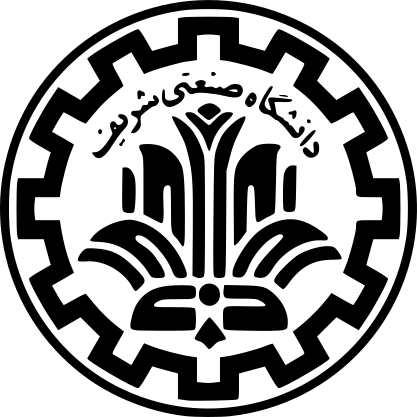
\includegraphics[scale=0.25]{logo.png}\\
		\vspace{0.5cm}
		\begin{Large}
			\textbf{
				دانشگاه صنعتی شریف\\
				\vspace{0.5cm}
				دانشکده مهندسی برق\\
			}
		\end{Large}
		\vspace{2.5cm}
		\begin{huge}
			\textbf{
				درس علوم اعصاب: یادگیری، حافظه، شناخت\\
				\vspace{1cm}
				تمرین مطالعاتی سری اول\\
			}
		\end{huge}
		\vspace{1.5cm}
		\begin{Large}
			\textbf{
				استاد درس: دکتر کربلایی آقاجان\\
				\vspace{1.5cm}
				امیرحسین افشارراد\\
				\vspace{0.5cm}
				۹۵۱۰۱۰۷۷\\
				\vspace{2cm}
				\today
			}
		\end{Large}
		
	\end{center}
	
	\thispagestyle{empty}
\end{titlepage}	

	\large
	\section{مقاله اول}
	\subsection{علل استفاده از تابع فعال‌سازی خطی یکسوشده}
	تابع فعال‌سازی خطی یکسوشده 
	\lr{(Rectified Linear Units - ReLU)}
	با توجه به ضابطه‌ی ساده‌تر خود (در مقایسه با توابع فعال‌سازی دیگری مانند \lr{sigmoid}) پیاده‌سازی روش 
	\lr{gradient-descent}
	را آسان‌تر می‌کنند؛ و به تبع آن باعث افزایش سرعت فرایند آموزش 
	\lr{(training)}
	می‌شود. ضمناً لازم به ذکر است که در عمل، مشاهده می‌شود که استفاده از این تابع فعال‌سازی نتایج عملیاتی بسیار خوبی دارد و این موضوع در کنار سرعت بالا، از علل استفاده از این تابع فعال‌سازی است.\\

	
	\subsection{مقایسه‌ی شبکه‌های عمیق و کم‌عمق}
	طبق تعریف، شبکه‌ی کم عمق شبکه‌ای است که تنها یک لایه‌ی پنهان داشته باشد، در حالی که شبکه‌ی عمیق بیش از یک لایه‌ی پنهان دارد. \\
	
	از نظر قدرت محاسبه، می‌توان گفت که هر دو نوع شبکه قادر به تخمین زدن هر تابعی هستند. شبکه‌ی کم‌عمق می‌تواند هر تابع پیچیده‌ای را به شکل یک تابع چندضابطه‌ای مدل کند؛ اما ممکن است تعداد ضوابط بسیار زیاد شود. ضمناً شبکه‌ی عمیق می‌تواند عملکردی دقیقاً مشابه با شبکه‌ی کم عمق را پیاده‌سازی کند.\\
	
	با این حال، تفاوت مهم این دو نوع شبکه آن است که شبکه‌ی عمیق قادر است توابع پیچیده را به شکلی \textbf{مختصرتر و با تعداد واحدهای محاسباتی کمتری }مدل کند. علت مهم این امر، آن است که شبکه‌ی عمیق می‌تواند خروجی‌های لایه‌های مختلف را (به صورت سلسله‌مراتبی) \textbf{مجدداً مورد پردازش }قرار دهد و نتایج را گسترش دهد؛ در حالی که این کار در شبکه‌ی کم‌عمق امکان‌پذیر نیست.
	
	\subsection{مقایسه‌ی شبکه‌های {feedforward} و {recurrent}}
	شبکه‌های مستقیم \lr{(feedforward)} تنها قادر به محاسبه و تخمین توابع استاتیک (غیر متغیر با زمان) هستند. در طرف مقابل، شبکه‌های بازگشتی \lr{(recurrent)} می‌توانند دینامیک متغیر با زمان سیستم‌ها را محاسبه کرده و تخمین بزنند و در لحظات مختلف، حالت سیستم را در خود نگه‌داری کنند. در این نوع شبکه‌ها، اتصالات تنها از یک لایه به لایه‌ی بعدی برقرار نیست، بلکه هر لایه می‌تواند اتصالاتی به خود، و نیز به لایه‌های قبلی داشته باشد. به این ترتیب، مفهوم لایه‌ها تقریباً معنای اصلی خود را از دست می‌دهند، چرا که می‌توان تمامی لایه‌های پنهان را به شکل یک لایه در نظر گرفت که درون خود دارای اتصالاتی است.\\
	
	برای تعیین وزن‌های هر دو نوع شبکه از روش انتشار به عقب \lr{(backpropagation)} استفاده می‌شود، و می‌توان شبکه‌های بازگشتی را نیز به نوعی مشابه با شبکه‌های مستقیم در نظر گرفت، تنها به این تفاوت که در بُعد زمان گسترش یافته‌اند. یک تفاوت قابل توجه در آموزش برخی از شبکه‌های بازگشتی 
	\lr{(echo-state networks)}
	آن است که وزن بین لایه‌های پنهان مورد آموزش قرار نمی‌گیرد و به صورت تصادفی انتخاب می‌گردد، تا اثر موج‌گونه‌ی ورودی متغیر با  زمان و الگوهای زمانی موجود در آن، در نهایت بر شبکه حاکم شود.
	\subsection{مفاهیم محو و انفجار گرادیان در شبکه‌های عصبی}
	در آموزش شبکه‌های عصبی بازگشتی \lr{(recurrent)}، بعضاً مشاهده می‌شود که مقدار گرادیان  بسیار کوچک یا صفر می‌شود (و جهت ادامه‌ی فرایند نامشخص می‌گردد، یا به عبارت دیگر وزن مورد نظر دیگر تغییر نمی‌کند و نمی‌تواند بهبود یابد) یا مقدار آن بسیار بزرگ می‌شود (منفجر می‌گردد).\\
	علت این امر آن است که برای یادگیری وابستگی‌های زمانی طولانی‌مدت در شبکه‌های بازگشتی، محاسبه‌ی گرادیان (از رابطه‌ی مشتق زنجیری) از حاصل‌ضرب تعداد زیادی عبارت محاسبه می‌گردد که امکان صفر یا بسیار بزرگ شدن را ایجاد می‌کند.\\
	
	برای حل این مشکل از ساختار 
	\lr{Long Short-Term Memory (LSTM)} 
	استفاده می‌شود. در این ساختار، واحدهای محاسباتی قادر به نگه‌داری خاطرات کوتاه‌مدت برای هر زمان طولانی و دل‌خواهی هستند که این امر باعث می‌شود حساسیت و مشکل ناشی از اختلاف زمانی طولانی بین الگوهای بامعنی از بین برود.
	
	\subsection{شباهت شبکه‌های مصنوعی تشخیص تصاویر با شبکه‌های زیستی مغز}
	در شبکه‌های مصنوعی پردازش‌گر تصویر، لایه‌های ابتدایی عملکردی مشابه با نورون‌های 
	\lr{V1 (primary visual cortex)}
	دارند. این لایه‌ها به خصوصیت‌هایی از جنس فیلترهای \lr{gabor} حساسیت دارند؛ یعنی الگوهای ساده‌ای به شکل بافت‌های تکرارشونده (مانند خطوط سیاه و سفید موازی با فرکانس مکانی ثابت) را تشخیص می‌دهند.
	
	\subsection{Attacks Adversarial}
	
	\begin{itemize}
		\item 
		برخی روش‌های دفاع در مقابل حمله‌های \lr{adversarial}:
		\begin{enumerate} [label=\arabic*-]
		\item 
		\lr{Network Distillation}\\
		در این روش تلاش می‌شود تا اطلاعات از شبکه‌ی عصبی اولیه به یک شبکه‌ی عصبی کوچک‌تر منتقل شود؛ و با کاهش حساسیت نسبت به تغییرات و اغتشاشات کوچک در ورودی، مقاومت شبکه‌ی عصبی در مقابل حملات \lr{adversarial} بیشتر شود.\\
		
		\item 
		\lr{Adversarial (Re)training}\\
		در این روش، در هر مرحله از فرایند یادگیری شبکه، مثال‌هایی از نوع \lr{adversarial} تولید شده و در میان داده‌های یادگیری قرار می‌گیرد تا فرایند آموزش شبکه‌ی عصبی شامل مثال‌های متنوعی از از نوع  \lr{adversarial} باشد و به این ترتیب، شبکه‌ی عصبی در نهایت نسبت به این نوع از ورودی مقاومت باشد.\\
		
		\item
		\lr{Adversarial Detecting}\\
		در این روش، یک شبکه‌ی کمکی جداگانه وظیفه‌ی تعیین \lr{adversarial} بودن یا نبودن را به عهده می‌گیرد، به گونه‌ای که پاسخ آن همواره به شکل باینری بوده و صرفاً مشخص می‌کند که آیا ورودی داده‌شده، مجاز است یا از نوع \lr{adversarial} می‌باشد. در این حالت، با استفاده از یک شبکه‌ی کمکی، تلاش می‌شود تا از ورود نمونه‌های \lr{adversarial} به شبکه‌ی اصلی به طور کلی جلوگیری شود.\\
		
		\item 
		\lr{Input Reconstruction}\\
		در این روش، با استفاده از رویکردهای مختلفی، سعی می‌شود تا با انجام یک تبدیل بر روی ورودی \lr{adversarial} آن را به یک ورودی سالم و مجاز تبدیل کنند. در این حالت، بعضاً شبکه‌های عصبی مجزایی آموزش داده می‌شوند تا ورودی‌های \lr{adversarial} را به ورودی‌های سالم تبدیل کرده و در ادامه، این ورودی‌های فیلترشده و سالم به شبکه‌ی اصلی وارد شوند.
		\lr{(denoising autoencoder networks)}\\
		
		\item 
		\lr{Network Verification}\\
		این روش تأکید بر مطالعه و شناخت دقیق شبکه‌ی عصبی آموزش‌داده‌شده دارد؛ به گونه‌ای که بتوان به صورت تئوری واکنش و رفتار آن را به ورودی‌های مختلف پیش‌بینی و مشخص کرد. در نتیجه، می‌توان مطمئن بود که رفتار شبکه در مقابل ورودی‌های \lr{adversarial} چگونه است و در صورت امکان، رفتار آن را بهبود بخشید؛ و اگر ممکن نیست، در مورد ورودی‌هایی که شبکه را به خطا می‌اندازند، آگاه باشیم.\\
		
		\item 
		\lr{Ensembling Defenses}\\
		این روش در واقع روش جدیدی نیست؛ و صرفاً بیان‌گر آن است که بهتر است برای مقاوم‌سازی  هرچه بیشتر شبکه‌های عصبی در برابر حملات \lr{adversarial} از ترکیب و ادغام چندین روش مختلف دفاعی (نظیر روش‌های مذکور) استفاده کنیم.\\
		
		\end{enumerate}
			مراجع:\\
			
\begin{latin}
		\begin{enumerate}
	\item 
	Xiaoyong Yuan, Pan He, Qile Zhu, Xiaolin Li, “Adversarial Examples: Attacks and Defenses for	Deep Learning”, 2018.
			
			\item 
			N. Papernot, P. McDaniel, X. Wu, S. Jha, and A. Swami, “Distillation
			as a defense to adversarial perturbations against deep neural networks,”
			in
			Security and Privacy (SP), 2016 IEEE Symposium on
			.   IEEE, 2016,
			pp. 582–597.
			
			\item 
			J. Goodfellow, J. Shlens, and C. Szegedy, “Explaining and harnessing
			adversarial examples,”
			arXiv preprint arXiv:1412.6572, 2014.

			
			\item
			J. Lu, T. Issaranon, and D. Forsyth, “Safetynet: Detecting and rejecting
			adversarial examples robustly,”
			ICCV, 2017.
			
			\item 
			J. H. Metzen, T. Genewein, V. Fischer, and B. Bischoff, “On detecting
			adversarial perturbations,”
			Proceedings of 5th International Conference
			on Learning Representations (ICLR), 2017.
			
			\item 
			 S.  Gu  and  L.  Rigazio,  “Towards  deep  neural  network  architectures
			robust   to   adversarial   examples,”
			Proceedings   of   the   International
			Conference on Learning Representations (ICLR), 2015.
			
		\item 
		G. Katz, C. Barrett, D. Dill, K. Julian, and M. Kochenderfer, “Reluplex:
		An  efficient  smt  solver  for  verifying  deep  neural  networks,”
		arXiv
		preprint arXiv:1702.01135
		, 2017.
		
		\item 
		 Y. Song, T. Kim, S. Nowozin, S. Ermon, and N. Kushman, “Pixelde-
		fend: Leveraging generative models to understand and defend against
		adversarial examples,”
		arXiv preprint arXiv:1710.10766
		, 2017.
	\end{enumerate}
\end{latin}	
	\item 
	روش‌های تولید تصاویری که علاوه بر شبکه‌های عصبی، انسان را نیز به اشتباه بیندازند:\\
	
	تولید تصاویر \lr{adversarial} به گونه‌ای که انسان را به اشتباه بیندازند، در مقایسه با حملات \lr{adversarial} عادی که شبکه‌ی عصبی مصنوعی را به اشتباه می‌اندازند، به مراتب پیچیده‌تر است. یک نکته آن است که اصولاً تعریف اولیه‌ی ما از این نوع تصاویر، مثال‌هایی است که اگر چه برای انسان واضح هستند و با تصویر اصلی تفاوتی نمی‌کنند، اما شبکه‌ی عصبی را به اشتباه می‌اندازند. با توجه به این توضیح، مثال‌های رایج و معروفی که برای خطای دید انسان وجود دارند نمی‌توانند پاسخ مناسبی برای این قسمت باشند، چرا که اصولاً هدف در این بخش تولید تصاویری است که اگر چه تفاوت خاصی با تصویر اولیه ندارند، اما اشبتاه طبقه‌بندی می‌شوند و همین هدف با توجه به توضیحات داده‌شده سؤال برانگیز است، چرا که اگر تعریف ما از عدم ایجاد تغییر خاص در تصویر معادل با درک انسانی باشد، دیگر نمی‌توان انتظار داشت که چنین تصویری درک انسانی را به اشتباه بیندازد!\\
	
	با همه‌ی این توضیحات، اگر به مقالات مراجعه کنیم و به بررسی پیاده‌سازی حملات \lr{adversarial} بر روی انسان بپردازیم، یک روش رایج آن است که مثال‌هایی از تصاویر \lr{adversarial} به دست آورند که قادر به فریب دادن تعداد قابل توجهی از شبکه‌های عصبی مصنوعی باشند. چنین مثال‌هایی احتمالاً بتوانند انسان را نیز دچار اشتباه کنند؛ اما یک نکته‌ی مهم آن است که برای انجام چنین آزمایشی باید زمان بسیار کوتاهی به فرد داد تا بین دو دسته تصمیم بگیرد (تا بررسی کنیم که آیا تصمیم درست است یا فرد فریب تصویر \lr{adversarial} را خورده است)، چرا که با گذشت زمان، تفاوت‌های بنیادین شبکه عصبی مصنوعی و طبیعی خود را نشان می‌دهند و فرد در بیشتر موارد قادر به تشخیص دسته‌بندی صحیح خواهد بود.\\
	
همان طور که گفته شد، تصاویری می‌توانند گزینه‌های احتمالی فریب انسان باشند که شبکه‌های عصبی متعددی را فریب داده باشند. ادعا می‌شود که در چنین تصاویری، نشانه‌هایی ظاهر می‌شود که توسط انسان نیز محسوس است. به عنوان مثال، شکل \ref{fig01} دو نمونه از چنین تصاویری را نشان می‌دهد. 
\begin{figure}[h!]
	\centering
	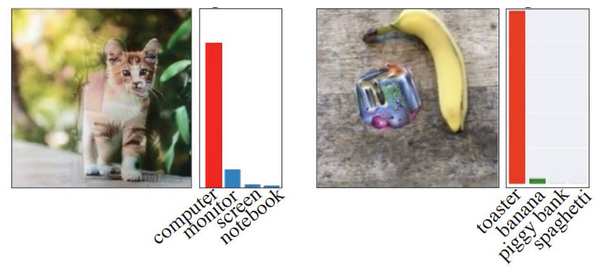
\includegraphics[scale=0.5]{fig01.png}
	\caption{نمونه‌هایی از تصاویری که قادر به فریب تعداد زیادی شبکه عصبی مصنوعی بوده و گزینه‌های احتمالی فریب انسان هستند}
	\label{fig01}
\end{figure}

تصویر سمت چپ گربه‌ای است که توسط شبکه‌های عصبی به عنوان کامپیوتر طبقه‌بندی می‌شود و تصویر دوم عکسی از یک موز است که توسط این شبکه‌ها به عنوان توستر طبقه‌بندی می‌شود. همان طور که گفته شد، نشانه‌هایی از لبه‌های تیز کامپیوتر در تصویر سمت چپ، و موجودی در وسط تصویر سمت راست که بی‌شباهت به توستر نیست، از جمله مواردی است که برای انسان محسوس است؛ با این حال در این مورد نمی‌توان ادعا کرد که انسان این تصاویر را به اشتباه تشخیص می‌دهد.\\

نمونه‌ی موجود در شکل \ref{fig02} بیشتر قابل اعتنا است. تصویر سمت چپ نشان‌دهنده‌ی یک گربه است، و تصویر سمت راست نیز همان گربه است اما با این تفاوت که عکس دچار حمله \lr{adversarial} شده است. در این حالت مشاهده می‌شود که امکان تشخیص اشتباه توسط انسان به مراتب قابل توجه است؛ به خصوص که (به دلایل ذکرشده) برای آزمایش انسان زمان بسیار کمی برای انتخاب یکی از دو طبقه‌بندی (سگ یا گربه) به وی می‌دهند، و مشاهده می‌شود که اشتباه در طبقه‌بندی بسیار زیاد است.

\begin{figure}[h!]
	\centering
	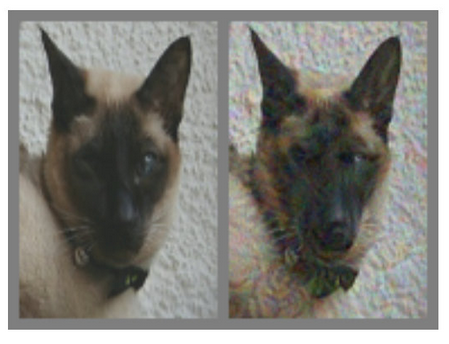
\includegraphics[scale=0.5]{fig02.png}
	\caption{تصویر چپ: تصویر اصلی گربه / تصویر راست: تصویر گربه پس از حمله \lr{adversarial} که به اشتباه به عنوان سگ طبقه‌بندی می‌شود}
	\label{fig02}
\end{figure}	
			مراجع:\\

\begin{latin}
	\begin{enumerate}
		\item 
		Gamaleldin F. Elsayed, 
		Shreya Shankar, 
		Brian Cheung, 
		Nicolas Papernot, 
		Alex Kurakin, 
		Ian Goodfellow, 
		Jascha Sohl-Dickstein, "Adversarial Examples that Fool both Computer
		Vision and Time-Limited Humans", 2018.
		
		\item 
\url{		https://spectrum.ieee.org/the-human-os/robotics/artificial-intelligence/hacking-the-brain-with-adversarial-images}
	\end{enumerate}
\end{latin}


	
	\end{itemize}
	
	\subsection{بررسی ناحیه‌ی IT در مغز و شباهت‌های آن با شبکه‌ها عصبی}
	ناحیه‌ی 
	\lr{IT(Inferior Temporal cortex)}
	معروف به طبقه‌بندی داده‌ها به گروه‌های مختلف است. این طبقه‌بندی کاری سطح بالاست و فراتر از تشخیص‌های الگو و فرایندهای پردازشی اولیه است؛ و در واقع کاری نظیر طبقه‌بندی محتوایی انجام می‌دهد.\\
	
	در مطالعات انجام‌شده مشاهده می‌شود که تنها شبکه‌های عصبی عمیق  (عمدتاً از نوع مبتنی بر کانولوشن) قادر به توجیه و مدل‌کردن رفتار \lr{IT} هستند و می‌توانند طبقه‌بندی‌های بین گروهی و درون‌گروهی مشابه با \lr{IT} را انجام دهند. همچنین مشاهده می‌شود که هر چه به  سمت لایه‌های بالاتر و عمیق‌تر این شبکه‌ها حرکت می‌کنیم، این مشابهت بیشتر می‌شود، و می‌توان گفت که تنهای لایه‌های بالایی (انتهایی) شبکه‌های عصبی عمیق می‌توانند عملکردی مشابه \lr{IT} داشته باشند.

	\clearpage

\section{مقاله دوم}
\subsection{ارجحیت مدل ارائه‌شده در مقایسه با مدل‌های معمول RNN}
تفاوت مشخص مدل ارائه‌شده در این مقاله با مدل‌های رایج مربوط به در نظر گرفتن نورون‌های \lr{excitatory} و \lr{inhibitory} است. اصولاً شبکه‌های عصبی متعددی می‌توانند با ساختارهای داخلی و دینامیک‌های متفاوت به نتایج یکسان (و صحیح) برسند. در این گونه موارد، مشاهده می‌شود که عملکرد و خروجی شبکه‌ی عصبی مصنوعی با آن‌چه که در واقعیت (و مثلاً در مغز انسان) اتفاق می‌افتد یکسان است، اما نحوه‌ی عملکرد داخلی آن‌ها ممکن است کاملاً متفاوت باشد. بدیهی است عملکرد داخلی چنین شبکه‌هایی نمی‌تواند برای شبیه‌سازی و شناخت بیشتر رفتار درونی مغز مناسب باشد، بنابراین برای رسیدن به این هدف جدید، باید شبکه‌هایی را مورد بررسی و آموزش قرار داد که از لحاظ عملکرد درونی نیز مشابه با شبکه‌های طبیعی عمل کنند.\\

با توجه به این توضیحات، ارزش کار این مقاله آن است که با ارائه‌ی مدلی مبتنی بر وجود نورون‌های \lr{excitatory} و \lr{inhibitory} قادر است شبکه‌های عصبی‌ای را تولید کند که علاوه بر ارائه‌ی خروجی‌های مطلوب، از نظر دینامیک داخلی نیز عملکردی مشابه با مغز را دارا باشند و بتوانند در بررسی و شبیه‌سازی رفتار داخلی مغز مؤثر واقع شوند.
\subsection{روش آموزش شبکه}
روش مورد استفاده در این مقاله، روش «کاهش گرادیان تصادفی» -
\lr{minibatch Stochastic Gradient Descent (SGD)}- 
است. علت استفاده از این روش، مزیت‌هایی است که در مقایسه با سایر روش‌های رایج دارد. در متن مقاله، این روش را با دو روش 
\lr{Hessian-Free (HF)} و \lr{First-Order Reduced and Controlled Error (Force)} 
مقایسه کرده‌اند. روش \lr{SGD} بر خلاف \lr{FORCE} (و مشابه با \lr{HF}) امکان فرمول‌بندی آسان مسأله‌ی آموزش \lr{RNN} را به صورت یک مسأله‌ی بهینه‌سازی تابع هدف در اختیار قرار می‌دهد، که با تغییر دادن آن می‌توان به جواب‌های مختلفی دست یافت. همچنین روش \lr{SGD} بر خلاف \lr{HF} (و مشابه با \lr{FORCE}) می‌تواند پارامترهای محاسبه‌شده را بعد از هر \lr{trial} به‌روزرسانی کند، و مجبور به دریافت تمامی داده‌ها در یک مرحله نمی‌باشد. به عبارت دیگر، امکان یادگیری به صورت آنلاین 
\lr{(online learning)} 
وجود دارد. بدین ترتیب، امکان بررسی اثرات بین آزمایشی 
\lr{across-trial}
به وجود می‌آید.\\

البته باید توجه داشت که هیچ‌کدام از روش‌های مذکور دقیقاً‌ آن‌چه در مغز اتفاق می‌افتد یکسان نیستد. روش مورد استفاده در مغز، 
\lr{Spike-Timing Dependent Plasticity (STDP)}
نام دارد که بر اساس آن، اتصالات بین نورون‌ها بر مبنای زمان‌بندی اسپایک زدن آن‌ها و سنکرون بودن این زمان‌بندی‌ها تنظیم می‌شود.

\subsection{چگونگی اضافه کردن نورون‌های excitatory و inhibitory به RNN های معمولی}
	مدل اصلی و ابتدایی شبکه در معادلات \ref{eq01} تا \ref{eq03} مشاهده می‌شود که در آن $\tau$ ثابت زمانی، $\mathbf{x}$ بردار جریان‌های ورودی، $W^{rec}$ ماتریس اتصالات بازگشتی
	 \lr{(recurrent)}،
	 $\mathbf{r}$ 
	 بردار
	 \lr{firing rate}، 
	 $\mathbf{z}$
	 بردار خروجی شبکه،
	  $W^{in}$ 	
	 ماتریس وزن ورودی،
	 $\mathbf{u}$
	 بردار ورودی‌های شبکه،
	  و $\boldsymbol{\xi}$ نویز است.
	
	\begin{equation}
			\tau \dot{\mathbf{x}} = -\mathbf{x}+W^{rec}\mathbf{r}+W^{in}\mathbf{u}+\sqrt{2\tau\sigma^2_{rec}}\boldsymbol{\xi} 
		\label{eq01}
	\end{equation}
	
		\begin{equation}
	\mathbf{r} = [\mathbf{x}]_+
	\label{eq02}
	\end{equation}

		\begin{equation}
\mathbf{z} = W^{out}\mathbf{r}
\label{eq03}
\end{equation}
برای تکمیل این مدل به منظور توجیه نورون‌های \lr{excitatory} و \lr{inhibitory}، باید به این نکته توجه داشت که اگر اتصال از نورون $j$ به نورون $i$ 
\lr{excitatory}
باشد، خواهیم داشت: 
$W^{rec}_{ij}>0$\\
همچنین اگر اتصال مذکور \lr{inhibitory} باشد، داریم: 
$W^{rec}_{ij}<0$\\
همچنین به طور کلی اگر نورون $j$ یک نورون \lr{excitatory} باشد خواهیم داشت: 
$\forall i : W^{rec}_{ij}\geq0$\\
همچنین در مورد نورون \lr{inhibitory} نیز به طریق مشابه داریم:
$\forall i : W^{rec}_{ij}\leq0$\\

حال برای کلی‌سازی مدل به منظور توجیه نورون‌های \lr{excitatory} و \lr{inhibitory}، ماتریس 
$W^{rec}$
را به شکل حاصل‌ضرب دو ماتریس دیگر در نظر می‌گیریم:
		\begin{equation}
W^{rec}=W^{rec,+}D
\label{eq04}
\end{equation}
که 
$W^{rec,+}$
ماتریسی نامنفی و $D$ ماتریسی قطری با مقادیر $1$ یا $-1$ است. هر عنصر از ماتریس ‌$D$ متناظر با یک نورون است که \lr{excitatory} یا \lr{inhibitory} بودن آن با $1$ یا $-1$ مشخص می‌شود. همچنین در اثر ضرب ماتریس‌ها، ماتریس 
$W^{rec}$ 
به دست می‌آید که ستون‌های متناظر با نورون‌های \lr{excitatory} همگی دارای مقادیر مثبت (یا صفر) و ستون‌های متناظر با نورون‌های \lr{inhibitory} همگی دارای مقادیر منفی (یا صفر) هستند: (در معادله \ref{eq05}، عناصر خالی معادل صفر هستند)
		\begin{equation}
\underbrace{\begin{bmatrix}
 & + & + & + & -\\
+  &  & + & + & -\\
 +  & + &  & + & -\\
  +  & + & + &  & -\\
   +  & + & + & + & \\
\end{bmatrix}
}_{W^{rec}}
=
\underbrace{\begin{bmatrix}
& + & + & + & +\\
+  &  & + & + & +\\
+  & + &  & + & +\\
+  & + & + &  & +\\
+  & + & + & + & \\
\end{bmatrix}
}_{W^{rec,+}}
\underbrace{\begin{bmatrix}
1&&&&\\
&1&&&\\
&&1&&\\
&&&1&\\
&&&&-1\\
\end{bmatrix}
}_{D}
\label{eq05}
\end{equation}

\subsection{مشکل انفجار گرادیان}
رابطه‌ی مورد استفاده در هر گام روش کاهش گرادیان در معادله \ref{eq06} مشاهده می‌شود. (
$\boldsymbol{\theta}$
بردار پارامترهای مدل است)
	\begin{equation}
		\boldsymbol{\theta^{(i)}} = \boldsymbol{\theta^{(i-1)}} + \boldsymbol{\delta\theta^{(i-1)}}
		\label{eq06}
	\end{equation}
که در آن، با محاسبه‌ی گرادیان گام بعدی به دست می‌آید:
\begin{equation}
	\boldsymbol{\delta\theta^{(i-1)}} = -\eta\nabla\mathcal{E}^{(i-1)}
	\label{eq07}
\end{equation}
در این روش، هنگامی که مقدار گرادیان بسیار بزرگ می‌شود (انفجار گرادیان)، روش مورد استفاده آن است که اصطلاحاً گرادیان را «می‌بُرند»، یا به عبارت دیگر اجازه‌ی عبور آن از یک مقدار مشخص $G$ را نمی‌دهند:
\begin{equation}
	\boldsymbol{\delta\theta^{(i-1)}} = \begin{cases}
	-\eta\nabla\mathcal{E}^{(i-1)}\times\frac{G}{|\nabla\mathcal{E}^{(i-1)}|}  & |\nabla\mathcal{E}^{(i-1)}|>G \\
	-\eta\nabla\mathcal{E}^{(i-1)}  & \text{otherwise }
\end{cases} \quad
	\label{eq08}
\end{equation}

\subsection{بررسی تسک‌های مختلف مبتنی بر مدل ارائه‌شده}
\subsubsection{تسک تصمیم‌گیری ادراکی}
این تسک مبتنی بر فرایند تصمیم‌گیری و انتخاب توسط شبکه‌ی عصبی است. این تصمیم‌گیری بین دو گزینه صورت می‌گیرد، به گونه‌ای که شواهدی در ارتباط با گزینه‌های موجود به شبکه ارائه می‌شود و در ادامه، شبکه‌ی عصبی باید یکی از این دو گزینه را (بر اساس شواهد) انتخاب کند. منظور از شواهد، دو تحریک، یکی مربوط به گزینه ۱ و دیگری مربوط به گزینه ۲ است. تحریک‌ها از آزمایش تشخیص حرکت تصادفی نقطه گرفته شده‌اند. ضمناً برای اعمال تحریک‌ها دو روش مختلف اتخاذ شده است؛ در روش اول دو تحریک برای مدت زمان معینی داده می‌شوند، سپس شبکه اقدام به تصمیم‌گیری می‌نماید؛ و در روش دوم تحریک‌ها برای زمانی نامحدود موجود هستند و شبکه در هر زمان قادر به تصمیم‌گیری است، اما سرعت واکنش شبکه نیز مورد بررسی و ارزیابی قرار می‌گیرد. ضمناً در هر دو حالت، در زمان ابتدایی آزمایش تحریکی وجود ندارد و انتظار داریم که خروجی شبکه‌ی عصبی در این زمان به ازای هر دو خروجی مقدار صفر (منظور از مقدار صفر، مقدار پایین یا به عبارت دیگر مقدار صفر منطقی است) داشته باشد. در ادامه و در زمان تصمیم‌گیری، شبکه با بالا بردن خروجی متناظر با گزینه‌ی مد نظر، آن گزینه را انتخاب می‌کند.\\

نتایج حاصل از این آزمایش قابل توجه هستند و عملکرد خوبی از شبکه‌های عصبی را به نمایش می‌گذارند. شکل  \ref{fig04} نتایج مختلفی از دو آزمایش را نشان می‌دهد که در ادامه به توضیح آن می‌پردازیم. دقت کنید که ستون سمت چپ مربوط به روش اول اعمال تحریک (با مدت زمان مشخص) و ستون سمت راست مربوط به روش دوم اعمال تحریک (با زمان نامتناهی) می‌باشد.

\begin{figure}[h!]
	\centering
	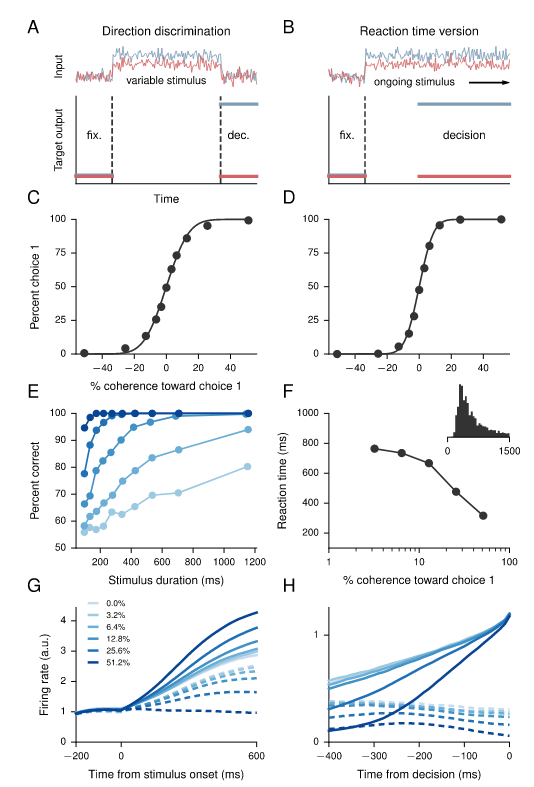
\includegraphics[scale=0.5]{fig04.png}
	\caption{نتایج آزمایش تصمیم‌گیری ادراکی}
	\label{fig04}
\end{figure}
پیش از توضیح نتایج، لازم به ذکر است که منظور از پارامتر 
\lr{coherence toward choice 1/2}
آن است که دو تحریک داده‌شده،‌ تا چه میزان تفاوت قابل توجهی میان دو انتخاب دارند، به گونه‌ای که هر چه مقدار این پارامتر (مثلاً در جهت گزینه ۱) بیشتر باشد، یعنی تحریک مربوط به این گزینه تفاوت معنادارتری نسبت به تحریک دیگر داشته و شواهد بیشتری برای انتخاب آن داریم.\\

شکل‌های A و B نشان‌دهنده‌ی فرایند انجام آزمایش هستند که پیش‌تر توضیح داده شد.\\

شکل‌های C و D درصد انتخاب گزینه ۱ را بر حسب \lr{coherence} در جهت این گزینه نشان می‌دهند، که می‌بینیم با افزایش 
\lr{coherence}
 در جهت این انتخاب، دقت پاسخ‌گویی نیز بسیار بالا می‌رود.\\
 
 شکل E درصد پاسخ صحیح را بر حسب مدت زمان اعمال تحریک (در روش اعمال تحریک با زمان محدود) نشان می‌دهد که نمودارهای مختلف آن مربوط به \lr{coherence}های متفاوت هستند. مشاهده می‌شود که در \lr{coherence}های بالا، تقریباً درصد پاسخ‌گویی شبکه مستقل از طول تحریک و در حدود $100\%$ است.\\
 
 شکل F زمان واکنش شبکه را بر حسب \lr{coherence} نشان می‌دهد. (برای روش دوم اعمال تحریک) که مشاهده می‌شود با افزایش \lr{coherence}، سرعت واکنش و تصمیم‌گیری شبکه افزایش می‌یابد.\\
 
 نهایتاً شکل‌های G و H نیز نشان‌دهنده‌ی 
\lr{firing rate}
بر حسب زمان اعمال تحریک می‌باشند. نمودارهای مختلف مربوط به \lr{coherence}های مختلف هستند که مجدداً مشاهده می‌شود \lr{coherence} بیشتر باعث عملکرد سریع‌تر و بهتر شبکه‌ی عصبی می‌شود.\\

نهایتاً به عنوان جمع‌بندی می‌توان گفت که عملکرد شبکه‌ی عصبی در انجام تصمیم‌گیری معقول و قابل قبول بوده و نتایج با انتظارات ما در تطابق نسبی هستند.


\subsubsection{تسک پارامتری حافظه‌ی کاری 
\lr{(Parametric working memory task)}
}
هدف از این تسک سنجش حافظه‌ی شبکه‌ی عصبی است، به گونه‌ای که مدتی پس از دریافت یک ورودی، بتواند آن را مورد بررسی و مقایسه قرار دهد. در این تسک، دو ورودی با فرکانس‌های متفاوت و با اختلاف زمانی مشخصی (حدود ۳ ثانیه) به شبکه‌ی عصبی داده می‌شوند، و سپس شبکه باید در خروجی، مشخص کند که فرکانس کدام ورودی بیشتر بوده است.\\

شکل \ref{fig03} درصد پاسخگویی این شبکه‌ی عصبی را در تشخیص فرکانس بالاتر بر حسب فرکانس‌های داده‌شده نشان می‌دهد؛ و مشخص است که نتایج قابل قبولی به دست آمده‌اند. ضمناً بنابر گزارش مقاله، تمامی درصدهای مشاهده‌شده بیشتر از $85\%$ بوده‌اند.

\begin{figure}[h!]
	\centering
	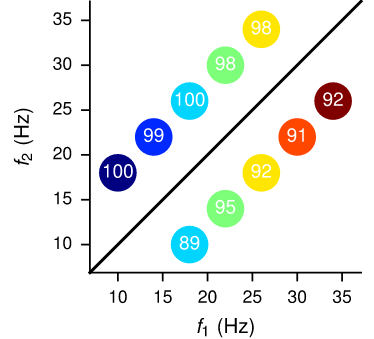
\includegraphics[scale=0.5]{fig03.png}
	\caption{درصد پاسخ صحیح شبکه‌ی عصبی در تشخیص فرکانس بالاتر}
	\label{fig03}
\end{figure}

\clearpage
\section{مقاله سوم}
\subsection{انواع کدهای نورونی}
\begin{itemize}
	\item 
	\lr{rate coding}:
	 در این روش کدگذاری، مبنای انتقال اطلاعات آهنگ (فرکانس) اسپایک‌زدن نورون‌ها است، و الگوی دقیق زمانی آن‌ها مد نظر نیست.
	 \item 
	 \lr{temporal coding}: 
	 در این روش کدگذاری، هنگامی که دقت زمانی بالایی مد نظر است؛ الگوی زمانی اسپایک‌ها و فاصله‌ی زمانی‌های آن‌ها در کد حامل اطلاعات است. 
\end{itemize}
به عنوان مثال، دو کد $000111000111$ و $00110011$ از منظر
\lr{rate coding}
یکسان هستند، چرا که آهنگ نوسان اسپایک‌ها در هر دو ثابت است؛ اما این دو از منظر 
\lr{temporal coding} 
متفاوت هستند، چرا که رفتار زمانی آن‌ها به وضوح متفاوت است.\\

رویکرد این مقاله در طراحی و مدل‌سازی، استفاده از مدل 
\lr{temporal coding}
بوده است.

\subsection{مدل‌سازی محاسباتی}
در مدل محاسباتی ارائه‌شده، برای نورون $j$، مجموعه $\Gamma_j$ نشان‌گر مجموعه‌ی نورون‌هایی است که به این نورون متصل هستند و اسپایک زدن آن‌ها بر نورون $j$ اثرگذار است؛ بنابراین نورون مورد نظر مجموعه‌ای از اسپایک‌ها را در زمان‌های $t_i$ دریافت می‌کند که $i\in\Gamma_j$.\\

در مدل ارائه‌شده، هر نورون در هر بازه‌ی شبیه‌سازی حداکثر یک اسپایک می‌زند، و شرط وقوع اسپایک نیز آن است که متغیر حالت داخلی این نورون به حد آستانه‌ی $\upsilon$ برسد. متغیر حالت مربوط به نورون $j$ تحت تأثیر اسپایک‌های ورودی قرار دارد، به گونه‌ای اثر آن از طریق یک تابع پاسخ اسپایک $\boldsymbol{\varepsilon}(t)$ اعمال می‌شود. همچنین  اثر هر کدام از اسپایک‌های ورودی به وسیله‌ی وزن $w_{ij}$ نیز تنظیم می‌شود، بنابراین به معادله‌ی \ref{eq09} دست خواهیم یافت.
\begin{equation}
x_j(t)=\sum_{i\in\Gamma_j}^{}w_{ij}\boldsymbol{\varepsilon}(t-t_i)
\label{eq09}
\end{equation}

همچنین تابع پاسخ اسپایک نیز از معادله  \ref{eq10}محاسبه می‌شود که در آن، منظور از $u(t)$ تابع پله واحد است و $\tau$ نیز ثابت زمانی نزول پتانسیل غشاء نورون است.
\begin{equation}
\boldsymbol{\varepsilon}(t)=\frac{t}{\tau}e^{1-\frac{t}{\tau}}u(t)
\label{eq10}
\end{equation}

همچنین برای تقویت مدل، هر اتصال بین نورونی را شامل $m$ اتصال سیناپسی در نظر می‌گیرند که هر ترمینال آن وزن و تأخیر متفاوتی دارد. معادله \ref{eq11} اثر هر ترمینال سیناپسی را (بدون در نظر گرفتن وزن) نشان می‌دهد.
\begin{equation}
y_i^k(t)=\boldsymbol{\varepsilon}(t-t_i-d^k)
\label{eq11}
\end{equation}
منظور از $d^k$ در معادله \ref{eq11} تأخیر ترمینال سیناپسی $k$ام است، که به معنی اختلاف زمانی اسپایک زدن نورون قبلی و زمان شروع به افزایش پتانسیل نورون مورد نظر است. شکل \ref{fig05} نشان‌گر این تأخیر است.
\begin{figure}[h!]
	\centering
	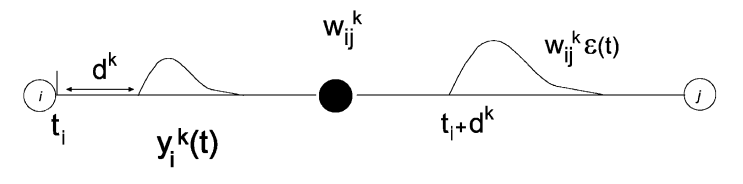
\includegraphics[scale=0.5]{fig05.png}
	\caption{تأخیر زمانی ترمینال‌های سیناپسی}
	\label{fig05}
\end{figure}

در نهایت برای تکمیل مدل، کافی است  اثر ترمینال‌های سیناپسی مختلف را در شکل‌دهی متغیر حالت در نظر بگیریم. معادله \ref{eq12} شکل کلی این مدل‌سازی را نشان می‌دهد.
\begin{equation}
x_j(t)=\sum_{i\in\Gamma_j}^{}\sum_{k=1}^{m}w^k_{ij}y^k_i(t)
\label{eq12}
\end{equation}

همچنین همان طور که پیش‌تر اشاره شد، شرط اسپایک زدن هر نورون آن است که مقدار متغیر حالت آن، از یک مقدار آستانه بیشتر شود؛ یعنی داشته باشیم 
$x_j(t)\geq\upsilon$
که مقدار $\upsilon$ برای تمامی نورون‌ها ثابت و مشترک است.


\subsection{backpropagation}
هدف از عملیات \lr{backpropagation} دستیابی به مجموعه‌ای از «زمان‌های اسپایک زدن» است. برای دستیابی به این هدف، وزن‌ها ($w_{ij}^k$) را در هر مرحله تغییر می‌دهند.\\

\begin{itemize}
	\item 
	یکی از چالش‌هایی که در فرایند \lr{backpropagation} و در این مدل به آن برمی‌خورند، آن است که ممکن است تغییرات ایجاد شده در وزن‌های مربوط به نورون به گونه‌ای به وقوع بپیوندند که پتانسیل غشاء نورون دیگر هیچ‌گاه به حد آستانه نرسد، و دیگر هیچ اسپایکی نزدند. در این صورت تخمین‌های مورد استفاده (تخمین مربوط به متغیر حالت $x_j$ و حد آستانه) دیگر معتبر نخواهند بود.\\
	 روش پیشنهادی برای حل این مشکل آن است که ورودی‌ها به گونه‌ای در شبکه کد شوند که اسپایک‌های زودهنگام به صورت اتوماتیک اهمیت بیشتری نسبت به اسپایک‌های دیرهنگام پیدا کنند.
	 
	 \item 
	 چالش دیگری که در این فرایند به وجود می‌آید آن است که اگر یک نورون برای هیچ الگوی ورودی اسپایک نزند، دیگر مکانیزمی برای تنظیم وزن‌های آن نورون وجود ندارد.\\
	 روشی که در این آزمایش برای حل این مشکل در نظر گرفته‌اند، آن است که وزن‌های ابتدایی هر نورون را به گونه‌ای تنظیم کرده‌اند تا حداقل به بخشی از الگوهای ورودی پاسخ بدهد. با این کار، دیگر مشکلی در ارتباط با نورون‌های خاموش مشاهده نشد.
\end{itemize} 

\subsection{کدگذاری متغیرها}
برای کدگذاری متغیرها با استفاده از روش زمانی 
\lr{(temporal coding)}
دو روش موجود است: اول استفاده از اختلاف زمانی‌های بسیار کم و رزولوشن زمانی بسیار بالا؛ و دوم استفاده از تعداد زیادی نورون به جای بالا بردن بیش از اندازه‌ی دقت زمانی.\\
با توجه به محدودیت‌های زیستی در مورد بالا بردن دقت زمانی و تلاش سازندگان مدل برای تعهد به این محدودیت‌ها، روش دوم را برای کد کردن ورودی انتخاب کرده‌اند؛ روش استفاده از جمعیت نورون‌ها.\\

برای کدگذاری در این روش از مفهوم  
\lr{receptive field (RF)}
 استفاده می‌شود. منظور از 
 \lr{receptive field}
  هر نورون، الگویی از ورودی است که نورون مربوطه به آن حساس است و در صورت مشاهده‌ی چنین الگویی در ورودی اسپایک می‌زند. بدیهی است نورون مد نظر در اثر ورودی‌های دیگر اسپایک نمی‌زند (یا به تعبیر دقیق‌تر، نرخ اسپایک زدن کمتری دارد).\\
  برای کدگذاری زمانی ورودی، نورون‌هایی که (با توجه به \lr{receptive field } خود) در اثر ورودی بیشتر برانگیخته می‌شوند، در زمان‌های زودتر، و نورون‌هایی که کم‌تر برانگیخته می‌شوند، در زمان‌های دیرتر اسپایک می‌زنند (یا به کلی اسپایک نمی‌زنند).\\
  
  نحوه‌ی کدگذاری خروجی در حالت طبقه‌بندی نیز از 
  \lr{winner-take-all paradigm}
   پیروی می‌کند؛ به این معنی که نورونی که نشان‌گر کلاس انتخابی طبقه‌بندی است زودتر اسپایک می‌زند، و تمامی نورون‌های مربوط به کلاس‌های دیگر با اختلاف زمانی معناداری دیرتر شروع به اسپایک زدن می‌کنند.
\end{document}

